\begin{figure}[htbp]
  \begin{center}
    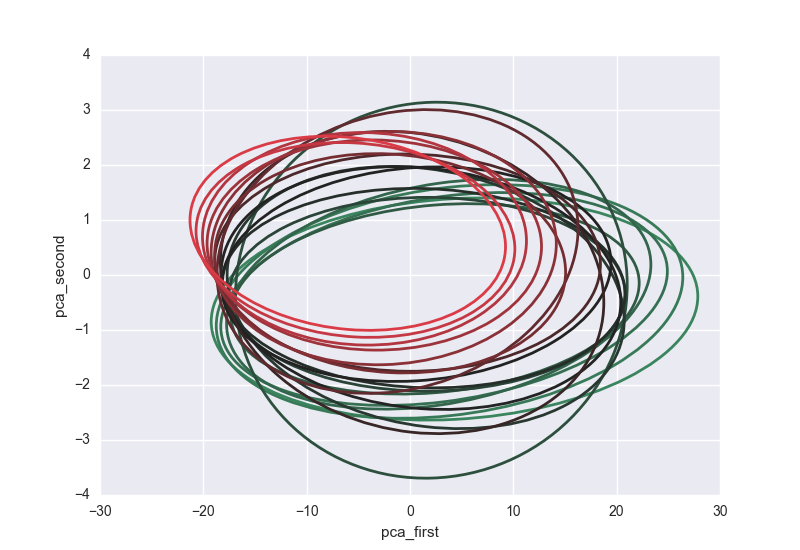
\includegraphics[clip,width=7.0cm]{fig/pca_gauss.png}
    \caption{主成分分析を行ったあとのデータ点から,各時刻ごとに二次元正規分布を求め,楕円としてプロットしたもの.楕円の大きさは,標準偏差の2倍になっている.緑から赤に近づくに連れて車線変更開始が近づいている.}
    \label{fig:pca_gauss}
  \end{center}
\end{figure}
